\documentclass[11pt]{article}

\usepackage{verbatim}
\usepackage{amsmath}
\usepackage{amssymb}
\usepackage{setspace}
\usepackage[top=1in, bottom=1in, left=1.25in, right=1.25in]{geometry}
\usepackage{subfigure}
\usepackage{graphicx}
\usepackage{cite}
\usepackage[squaren]{SIunits}
\usepackage{listings}
\usepackage{csquotes}

\setlength{\parindent}{0pt} 	% remove the silly paragraph indents

% Sample figure
%\begin{figure}[h!]
%\centering
%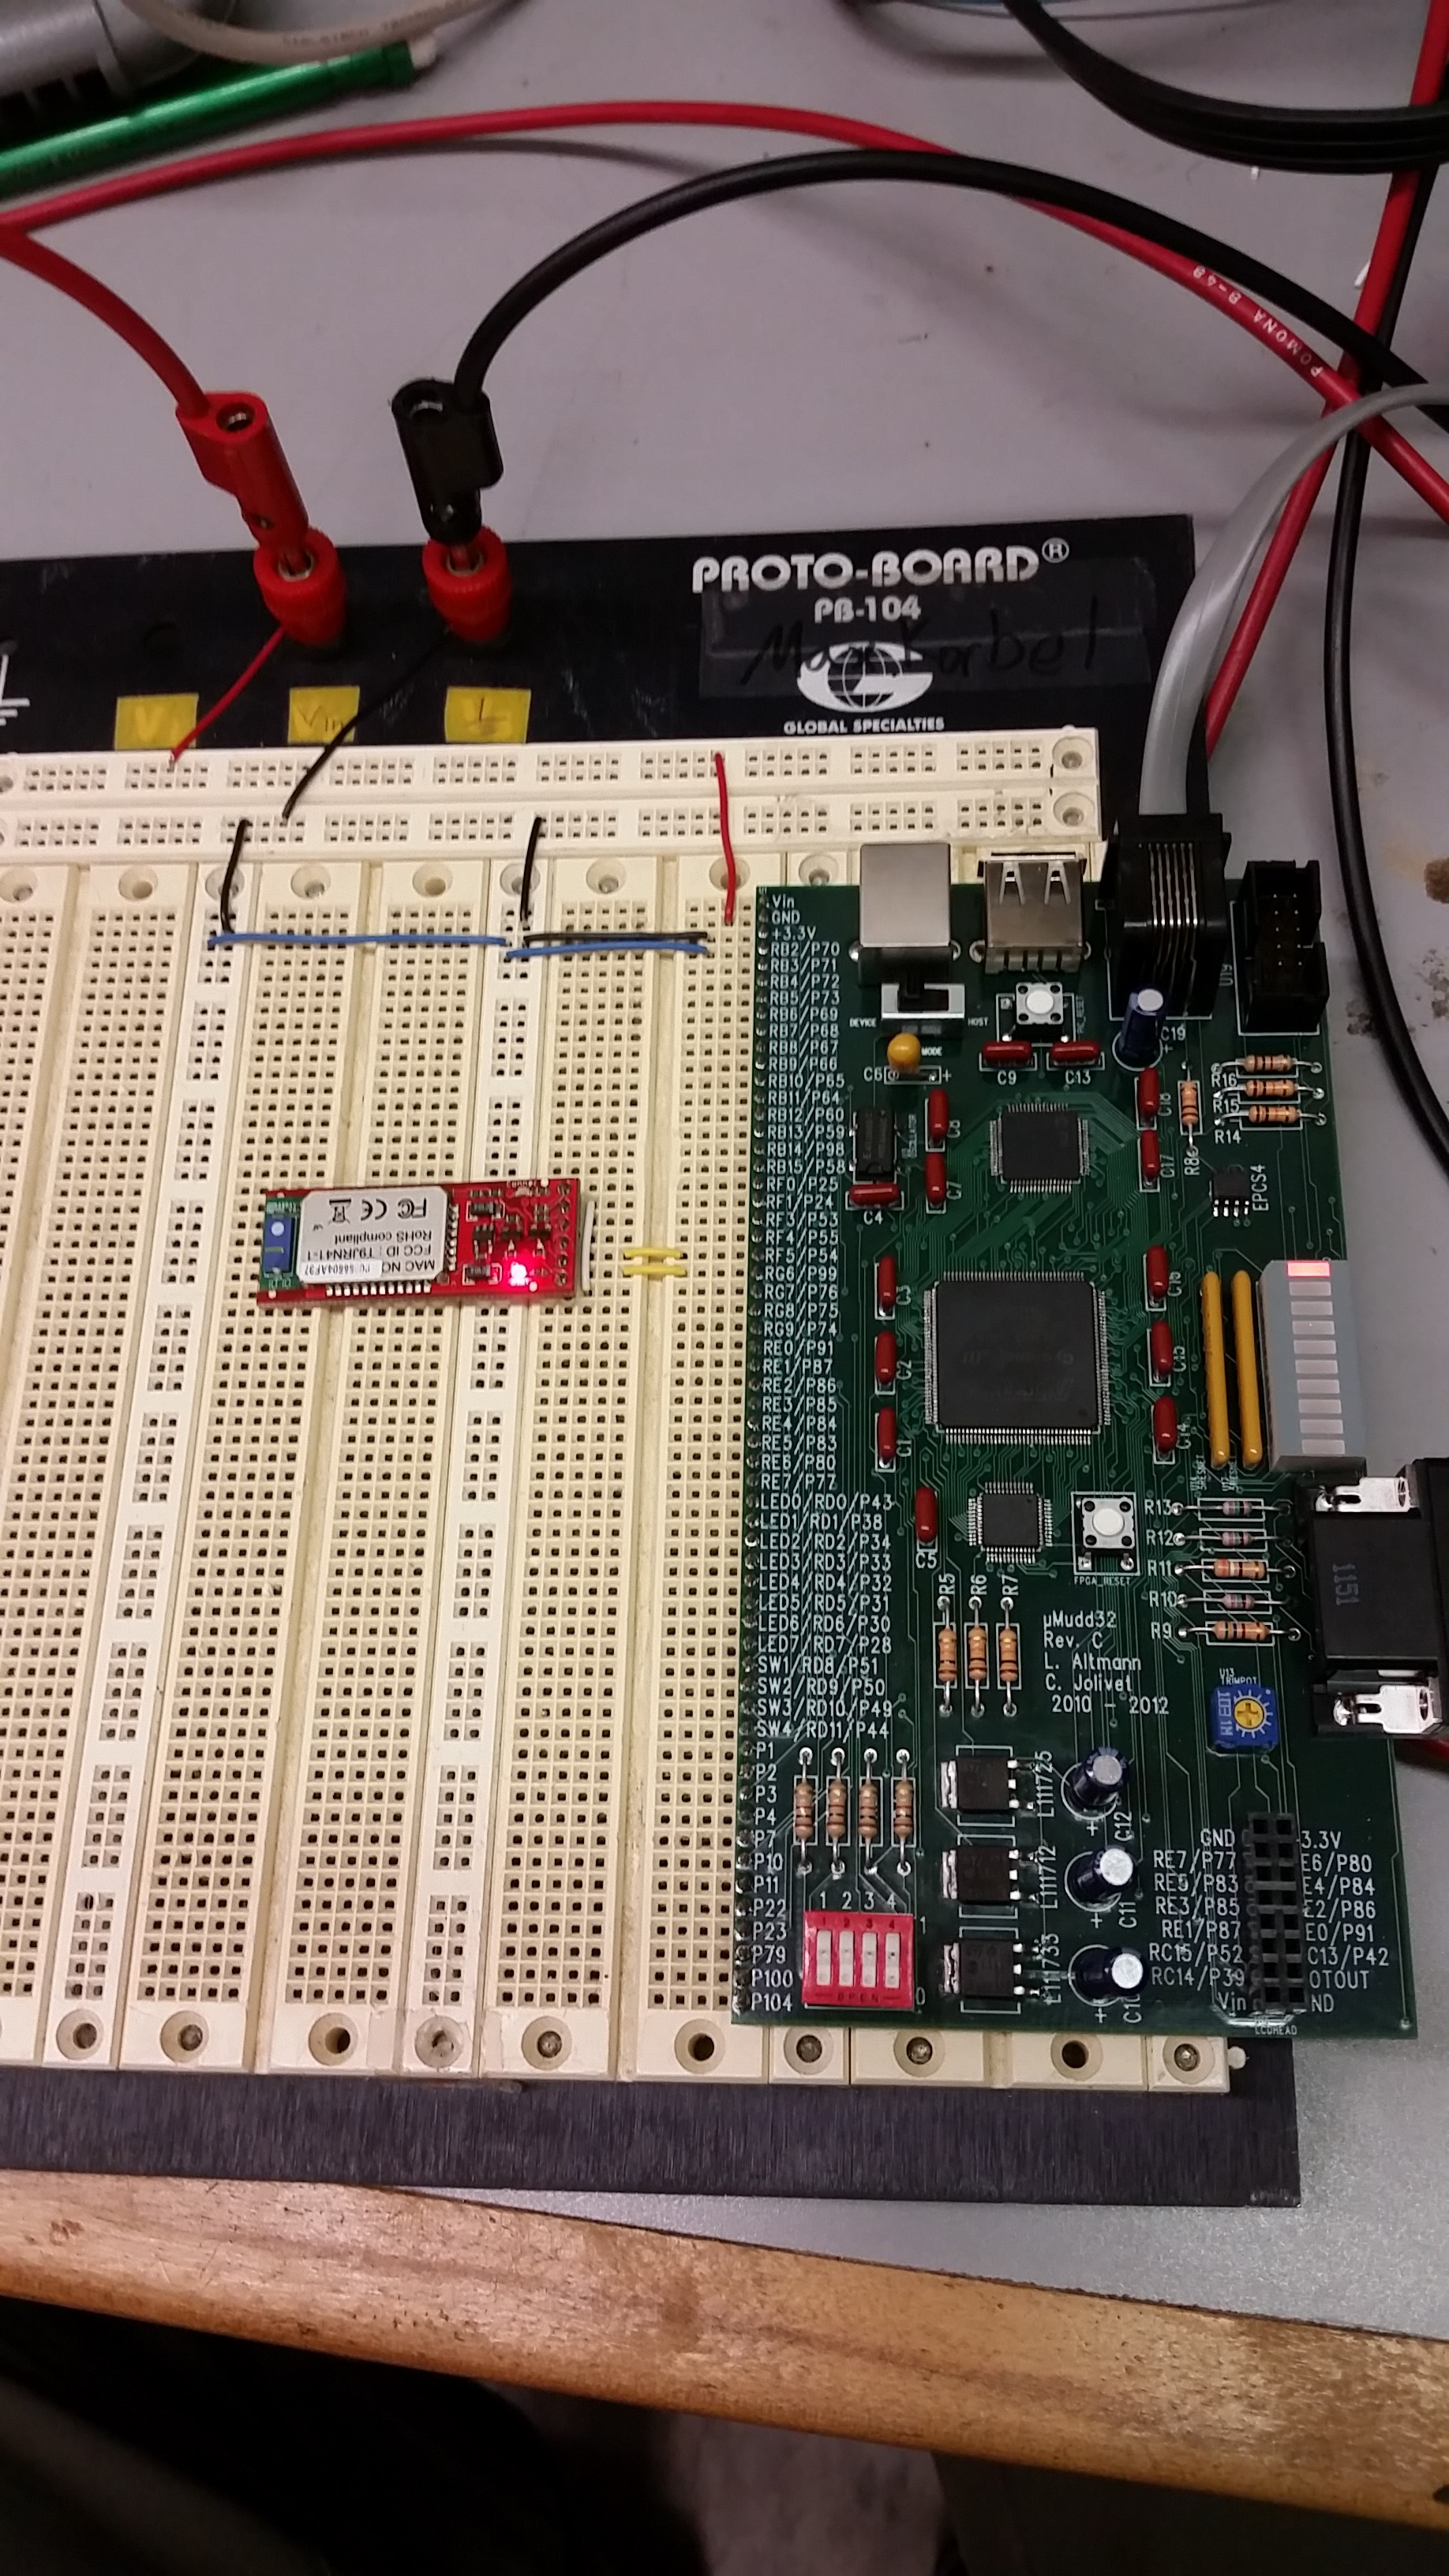
\includegraphics[scale=0.11]{board.jpg}
%\caption{The latest number entered on the keypad is displayed on the bottom display. The second latest number is displayed on the top.}
%\label{fig:board}
%\end{figure} 


\begin{document}



% ---------------------------------------
% Name section
% ---------------------------------------
\begin{flushleft}
Sherman Lam
\\E155
\\ \today
\end{flushleft}


% ---------------------------------------
% Title
% ---------------------------------------
\begin{center}
\begin{Large}
\textbf{Lab 7 Report: USB, SPI, and VGA}
\end{Large}
\end{center}


% ---------------------------------------
% Start report
% ---------------------------------------


\section{Introduction}
In this lab, I used both the PIC and FPGA on the $\mu$Mudd32 to create a mouse-to-monitor interface. The PIC interfaced with the mouse through USB. The FPGA interfaced with the monitor through VGA. The PIC and FPGA communicated through SPI. \\


\section{Design and Testing Methodology}

\begin{enumerate}
\item Using spi2
\item sclk - P99, sdo - P75, sdi - 76
\item vga already has pll setup
\item Pin assignments based on $\mu$Mudd32 pinout. \begin{verbatim} sync_b \end{verbatim} is sync (bar)
\end{enumerate}

\subsection{Mouse Tracking}
All mouse tracking functionality was performed on the PIC. The provided code reports the change in position of the mouse. I modified it to track the absolute x,y coordinates of the cursor and placed limits on the position to keep the cursor in the visible screen area (640x480). Each time the mouse is moved and the cursor position is updated, the new position is sent over SPI to the FPGA. \\

To make data transfer easy, the x and y coordinates are sent at the same time. The max value each coordinate can have is 640. This  can be represented in 10 or more bits. So, each coordinate is stored as a short (16-bits). A data packet consists of 32 bits. The bottom 16 bits are used to store the y coordinate while the top 16 bits are used to store the x coordinate. The data packet is then sent over SPI. \\

\subsection{SPI}
SPI is a serial data communication protocol and is commonly used to interface two digital systems. In each interface, there is a master - the device that performs the main job of managing the line of communication. The slave receives and send data when signaled by the the master. \\

In this lab, I used the PIC as the master since it has built in SPI peripherals and used the FPGA as the slave. The code I used was mostly based on SPI example code found in the class lectures. I used SPI2, which has the pinout from Table \ref{table:spi_pinout}.

\begin{table}[h!]
\centering
\begin{tabular}{|l|l|l|l|}
\hline
\multicolumn{4}{|c|}{\textbf{SPI Pin Mapping}} \\ \hline
\textbf{Signal}    & sclk    & sdo    & sdi    \\ \hline
\textbf{Pin}       & P99     & P75    & P76    \\ \hline
\end{tabular}
\caption{SPI 2 Pin Mapping}
\label{table:spi_pinout}
\end{table}

\textbf{sclk} is generated by the master and controls the timing of data transfer. \textbf{sdo} is the serial output pin for the master. That is, it transfers data from the master, to the slave. Finally, \textbf{sdi} is the serial input pin for the master. That is, it transfers data from the slave to the master. \\

On the PIC side, the baud rate was set to 1.25MHz. To send data through SPI, I just write the data (a 32-bit integer) to the SPI 2 buffer. Note that in order to send a 32-bit number, the MODE32 in the SPI 2 control register must be set to 1. \\

On the FPGA side, I used a simple shift register to receive data. Since the PIC doesn't need any information from the FPGA, the FPGA sends back 0s. \\

\subsection{VGA and displays on the FPGA}

All screen display functionality was handled by the FPGA. When a complete data packet is received through SPI, the data is parsed to obtain the x and y position of the cursor. Remember that the top 16 bits are used to store the x coordinate and the bottom 16 bits are used to store the y coordinate. \\

Two sets of RGB values are generated for the screen - one for the background and one for the cursor. The background image can be any pattern or color (see Section \ref{sec:gradient} to see how I defined a color gradient). The cursor image is black (RGB = 0,0,0) and white (RGB = 255,255,255). White corresponds to the image of the cursor while everything else is black. A final image with the cursor overlaid on top of the background can be obtained by performing a bitwise OR between the background and cursor images. \\

\subsection{Color Gradient Generation}
\label{sec:gradient}

The background I used consists of two gradients. The x axis features a gradient with increasing red content. The y axis features a gradient with increasing green content. The blue content is left 0 on the whole image. \\

The RGB values can range from 0 to 255. So, the gradient that maximizes this range would be defined by:

\begin{eqnarray*}
r = \frac{x}{640}255 \\
g = \frac{y}{480}255 
\end{eqnarray*}

However, it is difficult to implement division and multiplication in hardware. So, an alternative that provides nice results but doesn't fully utilize the range is:

\begin{eqnarray*}
r = x >> 2 \\
g = y >> 2
\end{eqnarray*}
 
Figure TODO shows the result of the gradient.

\subsection{Cursor Generation}

The cursor is just a 45-45-90 triangle with a short stem that in total forms an arrow. For a small 8x8 pixel area, the head is defined by x,y coordinates that follow the following constraint.
\begin{equation*}
x + y <= 8
\end{equation*}

The stem of the arrow is defined by the following constraint.
\begin{equation*}
x = y
\end{equation*}

However, when implemented on an area larger than the 8x8 pixel box, the constraints change slightly. Let $xpt$ and $ypt$ be the cursor position. For
\begin{eqnarray*}
	dx = x-xpt	\\
	dy = y-ypt
\end{eqnarray*}

The pixels in the arrow (head and stem) must follow these constraints:
\begin{eqnarray*}
	0 <= dx <= 8\\
	0 <= dy <= 8\\
	dx + dy <= 8\\
	dx = dy
\end{eqnarray*} 

\clearpage

\section{Technical Documentation}

\subsubsection{FPGA and PIC Pin Layout} 

Figures \ref{fig:fpga_sch} and \ref{fig:pic_sch} show parts of the $\mu$Mudd32 schematic that provide the needed pinouts.   

\begin{figure}[h!]
\centering
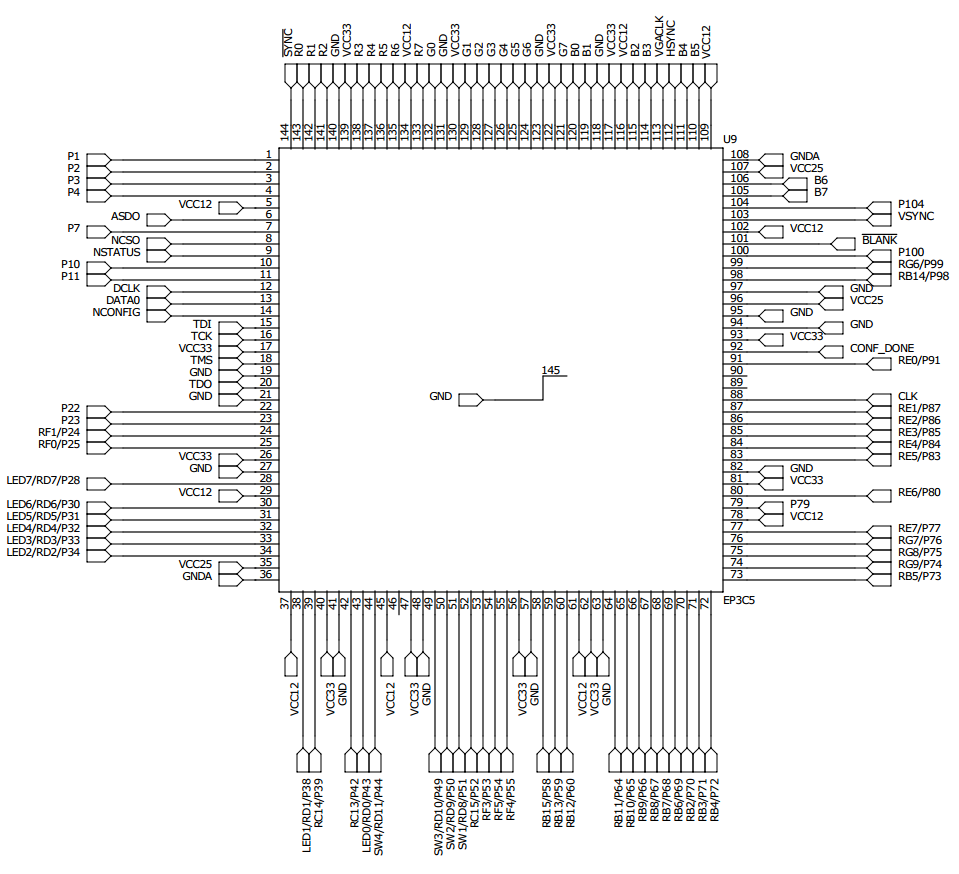
\includegraphics[scale=0.6]{fpga_sch.png}
\caption{FPGA pin layout. Pins that start with R,B,or G are RGB pins that are connected to the DAC.}
\label{fig:fpga_sch}
\end{figure} 


\begin{figure}[h!]
\centering
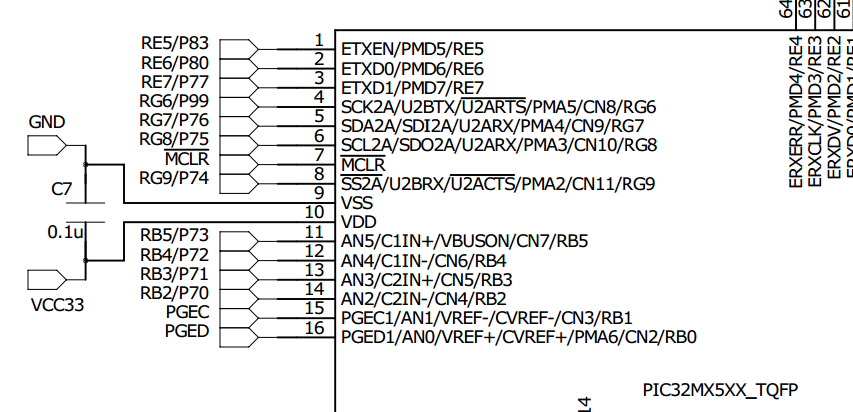
\includegraphics[scale=0.6]{pic_sch.png}
\caption{PIC pin layout. Relevant SPI 2 pins are SCK2A, SDI2A, and SDO2A.}
\label{fig:pic_sch}
\end{figure} 

\clearpage

\subsection{FPGA Code}
This section provides pieces of the code that I added to / modified from the provided FPGA VGA code.

\subsubsection{lab7\_SL.sv}

\begin{lstlisting}[numbers=left,language=verilog,basicstyle=\footnotesize]
module lab7_SL( input  logic        clk, reset,
                input  logic        sclk, sdo, sdi,         // spi communication lines      
                output logic        vgaclk,                 // 25 MHz VGA clock
                output logic        hsync, vsync, sync_b,   // to monitor & DAC
                output logic [7:0]  r, g, b);               // to video DAC
    
    logic [9:0] xpt;
    logic [9:0] ypt;
    logic ready;
    logic [31:0] data;
    //for displaying vga
    vga vga1(.clk(clk),.xpt(xpt),.ypt(ypt),
                .vgaclk(vgaclk),.hsync(hsync),.vsync(vsync),
                .sync_b(sync_b),.r(r),.g(g),.b(b));
    //for receiving spi data
    spiRx spi(.sclk(sclk),.sdo(sdo),.reset(reset),.ready(ready),
                    .sdi(sdi),.data(data));
    //for parsing data
    parse parser(.data(data),.reset(reset),.ready(ready),.xpt(xpt),.ypt(ypt));
endmodule


/*
Module for receiving 32 bit spi data

Author: Sherman Lam
Email: slam@g.hmc.edu
Date: 11-2-14
*/
module spiRx(   input logic         sclk, sdo, reset,   // SPI data lines
                output logic        sdi,                // SPI data
                output logic        ready,              // whether the data packet is ready
                output logic [31:0] data);              // data packet
    //counter for 32 bits
    parameter bits = 5'd31;
    logic [4:0] counter;
    
    //read on rising edge of spi clock
    always_ff@(posedge sclk) begin
        if (reset)  counter = '0;
        else            counter = counter + 1'b1; 
    end
    
    //shift register
    always_ff@(posedge sclk) begin
        data = {data[30:0],sdo};
    end
    
    assign ready = (counter == 0);
    
    //send back bogus data
    always_ff@(negedge sclk)
        sdi = 0;
    
endmodule


/*
Module for parsing spi data

Author: Sherman Lam
Email: slam@g.hmc.edu
Date: 11-2-14
*/
module parse(   input logic [31:0] data,        // data packet
                input logic ready, reset,       // whether data is ready to be stored, reset
                output logic [9:0] xpt, ypt);   // x and y position of cursor
    
    logic [31:0] dataCp;
    
    //store 32 bit data
    always_ff@(posedge ready, posedge reset) begin
        if (reset)      dataCp = '0;
        else            dataCp = data;
    end
    
    //mask to get x and y
    always_comb begin
        xpt = dataCp[25:16];
        ypt = dataCp[9:0];
    end
endmodule
\end{lstlisting}

\subsubsection{vga.sv}

\begin{lstlisting}[numbers=left,language=C,basicstyle=\footnotesize]

\end{lstlisting}

\clearpage


\section{Results and Discussion}

The cursor works as expected. The point of the cursor is design to not leave the 640x480 screen. However, if the cursor is on the 640 and/or 480 boundary, the body and stem of the arrow are allowed to exceed the bounded space. Only the very tip cannot leave. \\

The pin SYNC\_b in the provided VGA code corresponds with the pin $\overline{SYNC}$. 


\section{Conclusion}

\subsection{Time Spent}

\begin{description}
	\item[Programming] 6 hrs
 	\item[Writing Report] 2hrs
	\item[Total Time Spent] 8hrs
\end{description}

\subsection{Suggestions for lab}

Remove PLL section since it is in the provided VGA file. Or, put note that says ``This is for your interest only".
Provide pins for spi communications. \\ 

\end{document}

